\section{取样定理}

\subsection{信号的取样}

\begin{BoxDefinition}[理想取样]
    理想取样,又叫周期单位冲激取样,设取样脉冲为$s(t) = \delta_{T_s}(t)$,则
    \begin{Equation}
        s(t) = \delta_{T_s}(t) = \sum\limits_{n=-\infty}^{\infty} \delta(t-nT_s) \longleftrightarrow S(\mathrm{j}\omega) = \omega_s \sum\limits_{n=-\infty}^{\infty} \delta(\omega - n\omega_s)
    \end{Equation}
    则
    \begin{Equation}
        f_s(t) = f(t)\delta_{T_s}(t) = \sum\limits_{n=-\infty}^{\infty}f(nT_s)\delta(t-nT_s)
    \end{Equation}
    \begin{Equation}
        F_s(\mathrm{j}\omega) = \mathscr{F}\left[f(t)\delta_{T_s}(t)\right] = \frac{1}{2\pi}F(\mathrm{j}\omega)*\omega_s\delta_{\omega_s}(\omega) = \frac{1}{T_s}\sum\limits_{n=-\infty}^{\infty}F\left[\mathrm{j}(\omega-n\omega_s)\right]
    \end{Equation}
\end{BoxDefinition}


\begin{BoxProperty}[冲激取样信号的频谱]
    设$T_s$为取样间隔,$\omega_s$为取样角频率。当$\omega_s$满足下式时频谱不发生混叠,可以从$F_s(\mathrm{j}\omega)$中取出$F(\mathrm{j}\omega)$,即从$f_s(t)$中恢复原信号$f(t)$。
    \begin{Equation}
        \omega_s \geq 2\omega_m
    \end{Equation}
\end{BoxProperty}

\subsection{时域取样定理}

\begin{BoxTheorem}[时域取样定理]
    一个频谱在区间$(-\omega_m,\omega_m)$以外为$0$的带限信号$f(t)$,可唯一地由其在均匀间隔$T_s\left[T_s\leq\frac{1}{2f_m}\right]$上的样点值$f(kT_s)$确定。 
\end{BoxTheorem}

\begin{BoxProperty}[取样信号恢复原信号]
    理想低通滤波器
    \begin{Equation}
        H(\mathrm{j}\omega) = \left\{\begin{aligned}
            T_s & , & |\omega| < \omega_c \\
            0   & , & |\omega| > \omega_c
        \end{aligned}
        \right.
    \end{Equation}
    则将取样信号通过理想低通滤波器即可恢复原信号
    \begin{Equation}
        F(\mathrm{j}\omega) = F_s(\mathrm{j}\omega)H(\mathrm{j}\omega) \longleftrightarrow f(t) = f_s(t)*h(t)
    \end{Equation}
    其中$\omega_c$满足$\omega_m\leq\omega_c\leq\omega_s-\omega_m$
    \begin{Figure}[取样信号恢复原信号]
        \begin{FigureSub}[原始取样信号]
            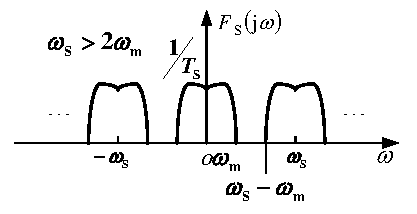
\includegraphics[width=50mm]{visio/4.14.pdf}
        \end{FigureSub}
        \begin{FigureSub}[理想低通滤波器]
            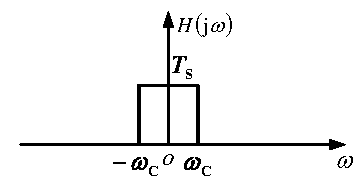
\includegraphics[width=40mm]{visio/4.14-b.pdf}
        \end{FigureSub}
        \begin{FigureSub}[原始信号频谱]
            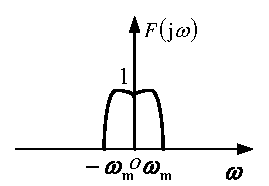
\includegraphics[width=30mm]{visio/4.14-c.pdf}
        \end{FigureSub}
    \end{Figure}
    即
    \begin{Equation}
        \begin{aligned}
            f(t) = f_s(t)*h(t) & = \left[\sum\limits_{n=-\infty}^{\infty}f(nT_s)\delta(t-nT_s)\right]*\left[T_s\frac{\omega_s}{\pi}\mathrm{Sa}(\omega_c t)\right] \\
                               & = T_s\frac{\omega_s}{\pi}\sum\limits_{-\infty}^{\infty}f(nT_s)\mathrm{Sa}\left[\omega_c(t-nT_s)\right]
        \end{aligned}
    \end{Equation}
    当$\omega_s=2\omega_m$,则$\omega_c = \omega_m$,$T_s = \frac{2\pi}{\omega_s} = \frac{\pi}{\omega_c}$,此时
    
    \begin{Equation}
        f(t) = \sum\limits_{n=-\infty}^{\infty}f(nT_s)\mathrm{Sa}\left[\omega_c(t-nT_s)\right]
    \end{Equation}
\end{BoxProperty}

\begin{BoxDefinition}[奈奎斯特频率与间隔]
    恢复原信号必须满足两个条件,一是$f(t)$必须是带限信号,二是取样频率不能太低,满足
    \begin{Equation}
        f_s\geq2f_m
    \end{Equation}
    或者取样间隔满足
    \begin{Equation}
        T_s\leq\frac{1}{2f_m}
    \end{Equation}
    否则会产生混叠。

    其中$f_s = 2f_m$称为奈奎斯特频率,$T_s = \frac{1}{2f_m}$称为奈奎斯特间隔。
\end{BoxDefinition}

